\documentclass[addpoints, 10pt]{exam}
\usepackage[T1]{fontenc}
\usepackage{amsmath}
\usepackage{amssymb}
\usepackage{systeme}
\usepackage{svg}
\usepackage{pgfplots}
\usepackage{bm}
\usepackage{multicol}
\usepackage{enumitem}
\usepackage{xcolor}
\usepackage{tikz}
\usepackage{float}
\usepackage[margin=2cm]{geometry}
\usepackage[most]{tcolorbox}
\usepackage{tabularx,booktabs}
\newcolumntype{Y}{>{\centering\arraybackslash}X}

\definecolor{gree}{RGB}{101, 191, 127}
\definecolor{gre}{RGB}{7, 135, 44}
\definecolor{crimson}{RGB}{220, 20, 60}
\definecolor{blu}{rgb}{0.34, 0.6, 0.7}
\definecolor{bl}{rgb}{0.34, 0.8, 0.8}
\pgfplotsset{width=10cm,compat=1.9}

\renewcommand{\arraystretch}{1.5}

\date{}
\title{MATH 4.1EL \\ Assignment 2 \\ (Quadratic Equations in One Unknown)}
\author{T Yeung}

\newtcolorbox{mycolorbox}[4]{colback=#2!10,enhanced,title=#1,
	attach boxed title to top left={xshift=-4mm},boxrule=0pt,after skip=0.3cm,before skip=0.5cm,right skip=0cm,breakable,fonttitle=\bfseries,toprule=0pt,bottomrule=0pt,rightrule=0pt,leftrule=4pt,arc=0mm,skin=enhancedlast jigsaw,sharp corners,colframe=#3,colbacktitle=#4,boxed title style={
		frame code={ 
			\fill[#4](frame.south west)--(frame.north west)--(frame.north east)--([xshift=3mm]frame.east)--(frame.south east)--cycle;
			\draw[line width=1mm,#4]([xshift=2mm]frame.north east)--([xshift=5mm]frame.east)--([xshift=2mm]frame.south east);
			\draw[line width=1mm,#4]([xshift=5mm]frame.north east)--([xshift=8mm]frame.east)--([xshift=5mm]frame.south east);
			\fill[#2!40](frame.south west)--+(4mm,-2mm)--+(4mm,2mm)--cycle;
		}
	}
}

\newtcolorbox{mycolorbox2}[2]{colback=#2!10,enhanced,title=#1,
	attach boxed title to top left={xshift=-4mm},boxrule=0pt,after skip=0.3cm,before skip=0.5cm,right skip=0cm,breakable,fonttitle=\bfseries,toprule=0pt,bottomrule=0pt,rightrule=0pt,leftrule=4pt,arc=0mm,colframe=#2,colbacktitle=#2, skin=enhancedmiddle  jigsaw
}

\renewcommand{\solutiontitle}{\noindent\textbf{\underline{Solution:}}\par\noindent}
\newenvironment{defin}[1]{\begin{mycolorbox}{Definition: #1}{green}{gree}{gre}}{\end{mycolorbox}}
\newenvironment{thm}[1]{\begin{mycolorbox}{Theorem: #1}{blue}{blu}{bl}}{\end{mycolorbox}}
\newenvironment{note}[1]{\begin{mycolorbox2}{Note: #1}{gray}}{\end{mycolorbox2}}
\newenvironment{mistake}[1]{\begin{mycolorbox2}{Common mistake: #1}{crimson}}{\end{mycolorbox2}}

\newcommand{\tf}[1][{}]{%
\fillin[#1][0.25in]%
}

\begin{document}
\maketitle

\begin{center}
	\fbox{\fbox{\parbox{5.5in}{\centering
				Answer the questions in the spaces provided on the
				question sheets. If you do not know how to answer 
				a certain question, write down where you get stuck.
				Answers can be corrected to 3 significant figures
				if necessary.
	}}}
\end{center}
\vspace{0.1in}
\makebox[\textwidth]{Name, class, class no.:\enspace\hrulefill}
\vspace{0.2in}
\makebox[\textwidth]{Tutor’s name:\enspace\hrulefill}

\begin{questions}

	\fullwidth{\section{Factorization of Polynomials}}
	\question Expand the following polynomials.
	\begin{multicols}{3}
		\begin{enumerate}[label=(\alph*)]
			\item $(x+y)^2$
			\item $(x-y)^2$
			\item $(x+y)(x-y)$
			\item $(x+y)(x^2-xy+y^2)$
			\item $(x-y)(x^2+xy+y^2)$
		\end{enumerate}
	\end{multicols}

	\question Expand the following polynomials
	\begin{multicols}{3}
		\begin{enumerate}[label=(\alph*)]
			\item $(3x+2y)^2$
			\item $(2x-3y)^2$
			\item $(3x+2y)(3x-2y)$
			\item $(2x+y)(4x^2-2xy+y^2)$
			\item $(2x-3y)(4x^2+6xy+9y^2)$
		\end{enumerate}
	\end{multicols}

	\question Factorize the following polynomials
	\begin{multicols}{3}
		\begin{enumerate}[label=(\alph*)]
			\item $x^2+9x+8$
			\item $4x^2+20x+25$
			\item $x^3-3x^2-10x$ 
			\item $(p+q)^2-9$
			\item $m(x+y)^2-4m(x-y)^2$
			\item $(x-1)^2+16(x-1)+64$
		\end{enumerate}
	\end{multicols}

	\fullwidth{\section{Solving Quadratic Equations}
		Quadratic equations are polynomials with the degree $2$. 
		To solve a quadratic equation, we rely on the following fact heavily:
		\begin{thm}{Product being 0 implies one of its factors must be 0}
			For any real numbers $m$ and $n$, if $mn=0$, then $m=0$ or $n=0$ (or both).
		\end{thm}
	}
	\newpage
	\question Solve the quadratic equation $(x+8)(x-1)=0$.
	\question Solve the quadratic equation $2x^2-x-3=0$.
	\question Solve the quadratic equation $x^2-6x=-9$.
	\question Solve the quadratic equation $81x^2=9$.
	\question Solve the quadratic equation $(7x-1)(3x-4)=5(7x-1)$.
	\fullwidth{\subsection{Graphical Method}}
	\begin{minipage}{\linewidth}
	\centering
		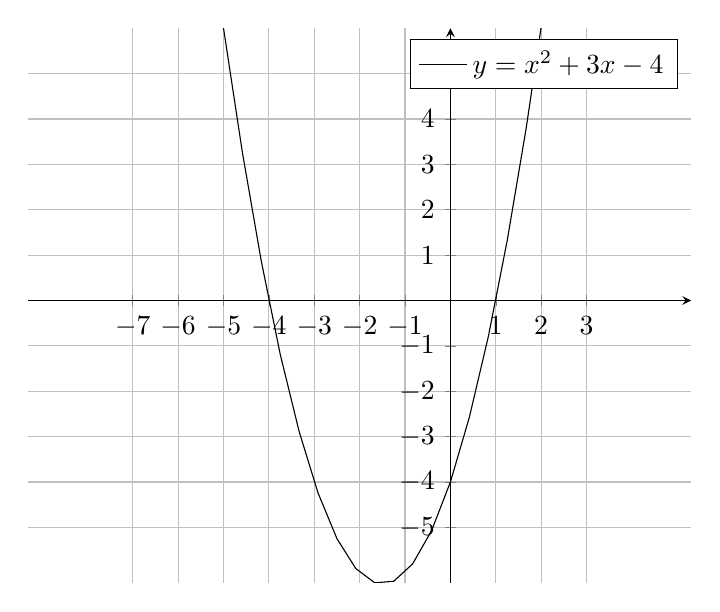
\begin{tikzpicture}
		\begin{axis}[
			axis y line = center,
			axis x line = middle,
			xmin=-6,xmax=2,
			axis equal,
			grid,
			ytick={-5,-4,..., 5},xtick={-7,-6,...,3}],
		]
		\addplot[mark=none]{x^2+3*x-4};
		\addlegendentry{$y=x^2+3x-4$}
		% \node[label={180:{$B(0,b)$}},circle,fill,inner sep=2pt] at (axis cs:0,3) {};
	\end{axis}
	\end{tikzpicture} \\
	\end{minipage}
	\question Given the above graph, how should we solve $x^2+3x-4=0$, how about 
	$\begin{cases}
		y=x^2+3x-4 \\
		y=\dfrac{1}{4}x-4
	\end{cases}$?
	Explain your reasoning behind your method.
	\question According to the graphical method, when will the equation $ax^2+bx+c=0$ have no solution? How about one and two solutions? ($a, b$ and $c$ are constants) Explain your answer in terms of the shape of the graph.
	\fullwidth{
		\subsection{Quadratic Formula}
		\begin{thm}{Quadratic formula}
			The roots of the quadratic equation $ax^2+bx+c=0$ (where $a\neq 0$) are given by the formula below
			\begin{equation*}
				x = \frac{-b \pm \sqrt{b^2-4ac} }{2a}
			\end{equation*}
		\end{thm}
	}
	\question Use the quadratic formula to solve the following quadratic equations.
	\begin{multicols}{2}
		\begin{enumerate}[label=(\alph*)]
			\item $x^2-4x-5=0$
			\item $6x^2+7x+2=0$
			\item $5x^2+6x-7=0$
			\item $3(2x+4)=3-5x^2$
			\item $(x+3)(x-3)=x(3x+4)$
			\item $5x^2+\frac{2}{5}=2 \sqrt{2} x$
		\end{enumerate}	
	\end{multicols}

	\newpage

	\fullwidth{\subsection{Discriminant}
		\begin{thm}{Discriminant}
			The discriminant, often denotes as $\Delta$ is the expression inside the surd in the quadratic formula.
			\begin{equation*}
				\Delta = b^2-4ac
			\end{equation*}
			\begin{tabularx}{\linewidth}{|X|X|X|X|}
				\hline
				Value of $\Delta$ & $\Delta > 0$ & $\Delta = 0$ & $\Delta < 0$ \\
				\hline
				Number of real roots & 2 & 1 & 0 \\
				\hline
			\end{tabularx}
		\end{thm}
	}
	
	\question Explain the why $\Delta$ has a relationship with the number of real roots.
	
	\question If the quadratic equation $kx^2+70x-25=0$ has two equal real roots, find the value of $k$.
	\question If the quadratic equation $7x^2-3(x+1)=k-x$ intersect with the x-axis, find the range of values of $k$.
	\question The base radius and the height of a solid right circular cylinder are $(9+x)$ cm and $(12-x)$ cm respectively.
	\begin{parts}

		\part Express the curved surface area of the cylinder in terms of $x$.

		\part If the curved surface area of the cylinder is $200\pi \text{cm}^2$, use the graph of $y=-x^2+3x+8$ to find the value(s) of $x$, correct to 1 decimal place. \\
		\begin{minipage}{\linewidth}
		\centering
			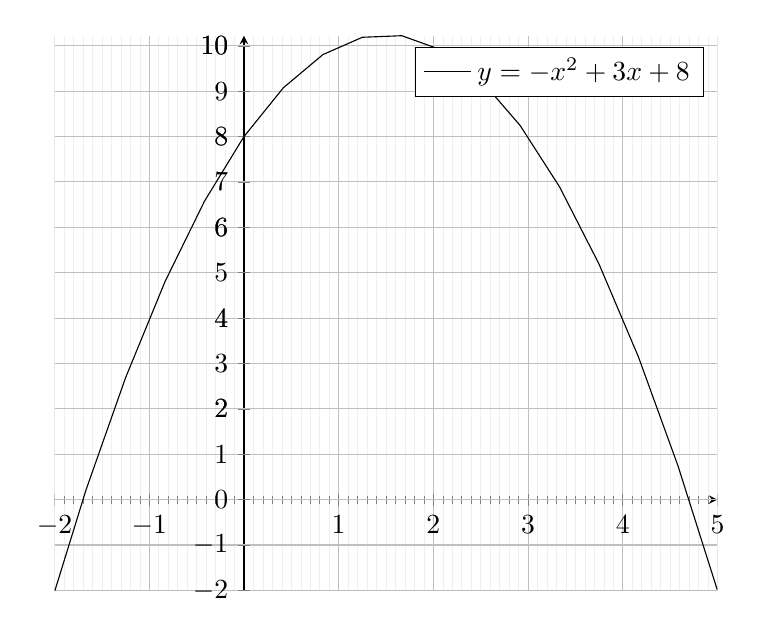
\begin{tikzpicture}
			\begin{axis}[
				grid=both,
				minor grid style={very thin, lightgray!25},
				axis y line = center,
				axis x line = middle,
				xmin=-2,xmax=5,
				minor x tick num = 9,
				extra y ticks={-2, -1, ..., 10},
				ytick={0, 2, ..., 10} ,xtick={-2,-1, ..., 5}
			]
			\addplot[mark=none]{-x^2+3*x+8};
			\addlegendentry{$y=-x^2+3x+8$}
			% \node[label={180:{$B(0,b)$}},circle,fill,inner sep=2pt] at (axis cs:0,3) {};
		\end{axis}
		\end{tikzpicture}
		\end{minipage}
	\end{parts}
	\question The following shows some patterns.
	\begin{figure}[H]
		\centering
		\includesvg[width=0.5\textwidth]{figures/pattern.svg}
		\caption{A pattern with dots}
	\end{figure}
	\begin{parts}
		\part Deduce a quadratic formula in $n$ for the number of dots in the $n^{\text{th}}$ figure.
		\part If the number of dots in the $m^{\text{th}}$ pattern is 506, find the value of $m$.
		\part If the total number of dots in the $k^{\text{th}}$ and $(k+2)^{\text{th}}$ pattern is $422$, find the value of $k$
		\part Is there a pattern with $307$ dots? Explain your answer.
	\end{parts}
	\question Given that the graph of $y=16px^2-8(3p+2)x-1$ touches the x-axis.
	\begin{parts}
		\part Find the two values of $p$
		\part For each of the values of $p$, solve the equation $16px^2-8(3p+2)x-1=0$.
	\end{parts}
	\question If the sum of two numbers is $36$ and the sum of their reciprocals is $\dfrac{1}{5}$, find the two numbers.
	\fullwidth{
		\begin{note}{Reciprocals}
			The reciprocal of a number $x$ is $\dfrac{1}{x}$, 
			for example, the reciprocal of $\dfrac{2}{3}$ is $\dfrac{3}{2}$.
		\end{note}
	}
	\question 
	\begin{parts}
		\part Solve the equation $2x^2+3x+1=0$.
		\part Hence, solve the equation $\dfrac{1}{y^2}+\dfrac{3}{y}+2=0$
	\end{parts}
	\fullwidth {
		\section{Relations between Roots and Coefficients}
		\begin{thm}{Sum of roots and Product of roots}
			For a quadratic equation $ax^2+bx+c=0$ with roots $\alpha$ and $\beta$,
			\begin{align*}
				\text{Sum of roots} = \alpha + \beta &=  -\frac{b}{a} \\
				\text{Product of roots} = \alpha\beta &= \phantom{-} \frac{c}{a}
			\end{align*}
		\end{thm}
		Determine whether the following statements are correct.
	}
	\question \tf The theorem is true for all complex roots $\alpha$ and $\beta$.
	\question \tf The theorem is true for quadratic equations with $\Delta < 0$.
	\question \tf $\alpha \neq \beta$
	\question \tf If $a > 0$ and $c > 0$, then $\alpha\beta > 0$
	\question Find the sum of roots and product of roots of the quadratic equation $3x^2+3x-5$. Also, find the solutions $\alpha$ and $\beta$ to verify the result.
	\question If $\alpha$ and $\beta$ are the roots of the equation $7x^2-2x-1=0$, find the value of each of the following expressions, assuming that $\alpha > \beta$
	\begin{multicols}{3}
		\begin{enumerate}[label=(\alph*)]
			\item $(3-\alpha)(3-\beta)$
			\item $\dfrac{\alpha}{\beta}+ \dfrac{\beta}{\alpha}$
			\item $7 \alpha^2 + 2 \beta$
			\item $\dfrac{1+2\alpha}{\alpha^3}+\dfrac{1+2\beta}{\beta^3}$
			\item $\alpha^2+\beta^2$
			\item $\alpha-\beta$
		\end{enumerate}
	\end{multicols}
	\newpage
	\fullwidth{
	\begin{mistake}{$a^2+b^2 \neq (a+b)^2$}
		\begin{equation*}
			a^2+b^2 \neq (a+b)^2 = a^2+2ab+b^2
		\end{equation*}
		Visualize it!
		\begin{figure}[H]
			\centering
			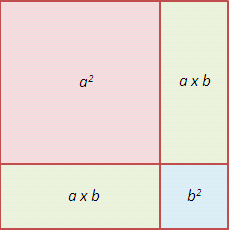
\includegraphics[width=0.3\textwidth]{figures/aplusbsquared.png}
			\caption{$(a+b)^2=a^2+2ab+b^2$}
		\end{figure}
	\end{mistake}
	}
	\question Form a quadratic equation in $x$ with roots $6+\sqrt{5}$ and $6-\sqrt{5}$.
	\question If $\alpha$ and $\beta$ are the roots of the equation $3x^2-5x-9=0$, form a quadratic equation in $x$ with roots $\alpha+2$ and $\beta-2$.
	\question $\alpha$ and $\beta$ are the roots of the equation $x^2-4x+2=0$, where $\alpha > \beta$.
	\begin{parts}
		\part Find the value of $\alpha-\beta$
		\part Form a quadratic equation in $x$ with roots $\dfrac{1}{\alpha}+\dfrac{1}{\beta}$ 
		and $\dfrac{1}{\alpha}-\dfrac{1}{\beta}$. (Leave the radical sign $\sqrt{}$ in the answers.)
	\end{parts}
	\question $\alpha$ and $\beta$ are the roots of the equation $x^2+3x-8=0$.
	\begin{parts}
		\part Find the value of $\dfrac{\beta}{\alpha}+\dfrac{\alpha}{\beta}$.
		\part Form a quadratic equation in $x$ with roots $\alpha-\dfrac{1}{\alpha}$ and $\beta  - \dfrac{1}{\beta}$.
	\end{parts}
	\newpage
	\fullwidth{\section{Exercises}}
	\begin{multicols}{2}
		\begin{minipage}{0.8\linewidth}
			\question If $\alpha \neq \beta$ and 
			$
			\begin{cases}
				3\alpha=\alpha^2-5 \\
				3\beta=\beta^2-5
			\end{cases}
			$,
			then $\alpha\beta=?$
			\begin{choices}
				\choice 3
				\choice -3
				\choice 5
				\choice -5
			\end{choices}
		\end{minipage}

		\begin{minipage}{0.9\linewidth}
			\question If the roots of the quadratic equation \\ $x^2-kx+3=0$ are $\alpha$ and $\beta$, then $\alpha^3+\beta^3=$

			\begin{choices}
				\choice $k^3$
				\choice	$k^3-3k$ 
				\choice $k^3-9k$
				\choice $k^3-12k$
			\end{choices}
		\end{minipage}

		\begin{minipage}{0.9\linewidth}
			\question If $\alpha$ and $\beta$ are unequal real numbers, and
			$
			\begin{cases}
				\alpha^2+12\alpha=2 \\
				\beta ^2 + 12 \beta \ = 2
			\end{cases}
			$
			, then $(3\alpha+1)(3\beta+1)=$

			\begin{choices}
				\choice $x=6$
				\choice $x=\dfrac{1}{6}$
				\choice $x=6 \text{ or } \dfrac{1}{6}$
				\choice $x=-6$
			\end{choices}
		\end{minipage}

		\begin{minipage}{0.9\linewidth}
			\question Solve the equation $x+\dfrac{1}{x} = 6+\dfrac{1}{6}$

			\begin{choices}
				\choice $x=6$
				\choice $x=\frac{1}{6}$
				\choice $x=6 \text{ or } \frac{1}{6}$
				\choice $x=-6$
			\end{choices}
		\end{minipage}

	
		\begin{minipage}{0.9\linewidth}
			\question Which of the following quadratic equations can be formed from the roots $-k$ and $\frac{1}{k} (k \neq 0$)
			\begin{choices}
				\choice $x^2+\left( \frac{1}{k}-k \right) x-1=0$	
				\choice $x^2+\left( k-\frac{1}{k} \right) x-1=0$	
				\choice $x^2+\left( \frac{1}{k}-k \right) x+1=0$	
				\choice $x^2+\left(k- \frac{1}{k} \right) x+1=0$	
			\end{choices}
		\end{minipage}

		\begin{minipage}{0.9\linewidth}
			\question Let $k$ be a constant. If the roots of the quadratic equation $x^2+4x+3k=0$ are $\alpha$ and $\beta$, then $4\alpha-\beta^2=^2$
			\begin{choices}
				\choice $3k-4$	
				\choice $3k+4$	
				\choice $3k-16$	
				\choice $3k+16$	
			\end{choices}
		\end{minipage}
	\end{multicols}
	\question If the equation $2x^2+(4k-1)x-k+\frac{5}{4}=0$ has no real roots in $x$, where $k$ is a constant, find the range of possible values of $k$.

	\question A piece of wire of length $42 \text{ cm }$ is cut into two parts and bent into a square and an equilateral triangle respectively. If the area of the square and that of the triangle are in the ratio $4:\sqrt{3}$, find the length of the side of the square. 

\end{questions}

\end{document}




